\chapter{Integrals of motion\label{chap:iom}}
\thispagestyle{chapterBeginStyle}

The problem of our interest is the systematic classification of all local and quasilocal integrals of
motion (LIOMs and QLIOMs) supported on up to \( M \in \NN \) sites in a model given by 1-D tight-binding Hamiltonian \(H\). 
To this end, we employ the algorithm first proposed in~\textcite{Mierzejewski2015a}. It allows us to classify integrals
of motions for a given system size \(L\). After doing so for accessible values of \(L\), we then carry out finite size scaling
to obtain information about the thermodynamic limit \(L \to \infty \). In principle this algorithm could
be also applied to lattice systems in two and more dimensions, however as of now it is prevented by computational
complexity of numerical approaches to such models.

In our description and used notation, we follow
the works of~\textcite{Mierzejewski2015a,Mierzejewski2015Approx,Mierzejewski2018}.
The aim of this chapter is to provide a pedagogical introduction to the topic,
so all derivations are presented in full detail, together with a simple proof of correctness of the algorithm.
The importance of (Q)LIOMs is be made clear by invoking the concepts of spectral functions and Mazur bound.
Examples of application of this algorithm to the XXZ model conclude this chapter.

The algorithm introduced in this chapter was implemented in C++ with the help of Armadillo
linear algebra library~\autocite{Sanderson2016,Sanderson2018}.

%%%%%%%%%%%%%%%%%%%%%%%%%%%%%%%%%%%%%%%%%%%%%%%%%%%%%%%%%%%%%%%%%%%%%%%%%%%%%%%%%%%%%%%%%%%%%%%%%%%%%%%%%%%%%%%%%%%%%%%%%%%%%%%%
\section{Preliminaries\label{sec:prelim}}
\paragraph{Space of observables}Consider the vector space \(\mathcal{V}_L\) of traceless and translationally invariant
observables, acting on a Hilbert space of dimension \(\dimension\). We can define an inner product on this space
\begin{definition}[Hilbert-Schmidt product]
  Let \(A,B \in \mathcal{V}_L\). The Hilbert-Schmidt product of \(A\) and \(B\) is
  \begin{equation}
    \hs{A}{B} = \frac{1}{\dimension}\tr(A^{\dagger}B) = \frac{1}{\dimension} \sum_{mn} A_{nm}B_{nm}^{\ast}
  \end{equation}
  where \(A_{nm} = \matrixel{n}{A}{m}\) and \(\ket{n},\ket{m}\) are eigenstates of some Hamiltonian,
  i.e.\ \(H\ket{n} = E_n \ket{n}\).
  Moreover, we define the Hilbert-Schmidt norm of an operator to be \(\norm{A} = \sqrt{\hs{A}{A}}\).
\end{definition}
The presented definitions are correct, as we work only with finite dimensional Hilbert spaces and taking
the trace is a linear operation. We require the operators to be traceless, because they have zero 
overlap with the identity, \(\left(A|\Id\right)=\frac{1}{D}\tr(A) = 0\).
Recall from statistical physics, that the average of an observable \(A\) over a canonical ensemble
in a finite temperature is given by
\begin{equation}
  \langle A \rangle_{\beta} = \frac{\tr(\mathrm{e}^{-\beta H}A)}{\tr(\mathrm{e}^{-\beta H})}
\end{equation}
where \(\beta = \frac{1}{kT}\).
Taking the limit \(\beta \to 0\), we obtain that \(\hs{A}{B} =  \langle AB \rangle_{0}\).
Therefore, the Hilbert-Schmidt inner product corresponds to the infinite temperature 
limit of averaging over a suitable ensemble (either canonical or grand canonical).
Now, consider a subspace \(\mathcal{V}_L^m\) of \(m\)-local operators and a direct sum
\(\mathcal{V}_L^M = \bigoplus_{m = 1}^M \mathcal{V}_L^m\) being a subspace of operators supported on up to \(M\) sites.
We define a basis of \(\mathcal{V}_L^M\) consisting of operators \(O_s\in \mathcal{V}_L^M\)
satisfying the following properties
\begin{align}
   & \hs{O_s}{O_{t}} = \delta_{st} \tag{\text{orthonormality}}                                    \nonumber{}\\
   & \big(\forall A \in \mathcal{V}_L^M\big) \big(A = \sum_s \hs{O_s}{A} O_s\big) \tag{\text{completeness}}   \nonumber{}\\
   & \big(\forall A \in \mathcal{V}_L \big) \big( A = A^M + A^{\perp} = \sum_s \hs{O_s}{A} O_s + A^{\perp}\big) ,
  \text{ such that } \big(\forall s\big) \Big( \hs{O_s}{A^{\perp}} = 0\Big)\label{eq:basis}
\end{align}


\paragraph{Locality} We begin with a definition of an integral of motion in quantum mechanics.
\begin{definition}
  Let \(H\) be a Hamiltonian operator. Then, any observable \(A\) commuting with the Hamiltonian
  \begin{equation*}
    \comm{H}{A} = 0
  \end{equation*}
  is an \textbf{integral of motion}.\label{def:iom}
\end{definition}
It is easy to see that there are many such observables. Let us consider the following
\begin{example}
  Take \(H\) to be any Hamiltonian operator. By spectral theorem, it can be written in diagonal form
  \begin{equation*}
    H = \sum_n E_n \ketbra{n}{n}
  \end{equation*}
  Then the set of projection operators \(P_n = \ketbra{n}{n}\) is a family of IOMs.
  However, the eigenstates of a Hamiltonian are in general very nonlocal.\label{ex: projectors}
\end{example}
However, as it will become evident in Section~\ref{sec:spectral function} on spectral functions, nonlocal operators are not important in the
thermodynamic limit and we are only interested in the so-called local (or quasilocal) integrals of motion.
A working intuition behind local operators is perhaps best seen in Figure~\ref{fig:1D chain}. They can be thought of as
being different from identity only on \(m\) consecutive sites. The XXZ Hamiltonian defined by equation~\eqref{eq:XXZ} is an
example of 2-local operator. On the other hand, a quasilocal operator can be represented as a convergent sum of operators
with increasing support.
\begin{figure}[!htbp]
  \centering
  \hspace*{-0.5cm}
  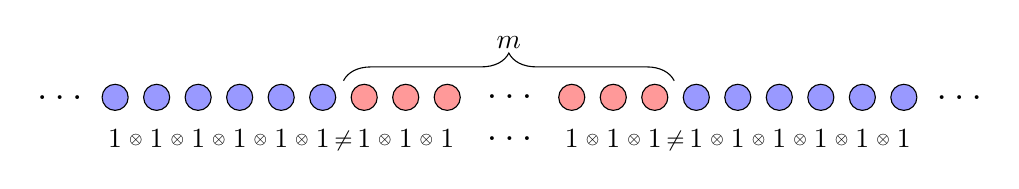
\begin{tikzpicture}[node distance = 15pt, auto]
    \tikzstyle{line} = [draw, -latex',thick]
    \tikzstyle{site1}=[circle, draw, fill=blue!40]
    \tikzstyle{site2}=[circle, draw, fill=red!40]
    % Place nodes

    \node [site1] (site-1) at (-8, 0) {};
    \foreach \x / \name in {1/2,2/3,3/4,4/5,5/6}
    \node [site1, right of=site-\x] (site-\name) {};

    \node [site2, right of =site-6] (site-7){};
    \foreach \x / \name in {7/8,8/9}
    \node [site2, right of=site-\x] (site-\name) {};

    \node [site2, right of=site-9, node distance=45pt] (site-10){};
    \foreach \x / \name in {10/11,11/12}
    \node [site2, right of=site-\x] (site-\name) {};

    \node[site1, right of=site-12] (site-13){};
    \foreach \x / \name in {13/14,14/15,15/16,16/17,17/18}
    \node [site1, right of=site-\x] (site-\name) {};

    \node [left of=site-1, node distance=20pt] {\Large $ \ldots $};
    \node [right of=site-18, node distance=20pt] {\Large $ \ldots $};


    \foreach \x in {1,...,18}
    \node [black, below of=site-\x](op-\x) {\(\mathbb{1}\)};

    \foreach \x / \y in {1/2,2/3,3/4,4/5,5/6,7/8,8/9,10/11,11/12,13/14,14/15,15/16,16/17,17/18}
    \path[draw=none] (op-\x) -- (op-\y) node [black,midway,yshift=-6pt] {\tiny$\otimes$};

    \path[draw=none] (op-6) -- (op-7) node [black,midway,yshift=-8pt] {\footnotesize$\neq$};
    \path[draw=none] (op-12) -- (op-13) node [black,midway,yshift=-8pt] {\footnotesize$\neq$};
    % \foreach \x in {-1.5,-1.0,-0.5,0.5,1.0,1.5}
    % \node [site2] (site-\x) at (\x, 0) {};

    \draw [decorate,decoration={brace,amplitude=10pt},yshift=6pt]
    (-5.1,0) -- (-0.9,0) node [black,midway,yshift=8pt] {$m$};

    \path [draw=none] (site-9) -- (site-10) node [black,midway,yshift=-4pt] {\Large$\ldots$};
    \path [draw=none] (op-9) -- (op-10) node [black,midway,yshift=-4pt] {\Large$\ldots$};
  \end{tikzpicture}
  \caption{Illustration of an operator supported on \(m\) sites.}\label{fig:1D chain}
\end{figure}
In Section~\ref{sec:algorithm}, a more precise definition of locality and quasilocality will be stated.

\paragraph{Noncommutativity}In the case of XXZ model, the Hamiltonian preserves total \(z\)-component of spin,
or in other words, it commutes with the total spin operator of the form
\begin{equation}
  \Sz_{tot} = \sum_{j = 1}^{L} \Sz_j
  \label{eq:magnetization}
\end{equation}
The resulting \(U(1)\) symmetry allows us to decompose the full Hilbert space into parts consisting of states with the same total \(z\)-component
of spin. In more mathematical terms, we have the following
\begin{equation*}
  \mathcal{H} = \bigoplus_{j = 0}^{L} \mathcal{H}_j \text{, where } \big(\forall \ket{\psi} \in \mathcal{H}_j \big) \big(\Sz_{tot} \ket{\psi} = \frac{1}{2}(2j-L) \ket{\psi} \big)
\end{equation*}
i.e.\;the full Hilbert space with \(\dim{\mathcal{H}} = 2^L\) can be decomposed into the direct sum of its proper subspaces
\(\mathcal{H}_j\) such that \(\dim{\mathcal{H}_j} = \binom{L}{j}\) and all states in a given subspace correspond to the same
eigenvalue of \(\Sz_{tot}\) operator. The index \(j\) denotes the number of sites with spin up.
Now we are ready for
\begin{definition}
  Let \(O\) be an integral of motion. If \(O\) preserves total \(z\)-component of spin, i.e.
  \(\comm{\Sz_{tot}}{O} = 0\), then it is called a \textbf{commuting integral of motion}.
  Otherwise, it is called a \textbf{noncommuting integral of motion}.\label{def:noncomm def}
\end{definition}
For the algorithm described in Section~\ref{sec:algorithm}, we need to construct matrices of
observables and express them in the Hamiltonian eigenbasis. If the operator in question is a
commuting IOM, we can restrict ourselves to the fixed spin subspace and thus greatly reduce
computational complexity, allowing us to investigate larger systems. Such operators, for example
spin energy current, have already been studied~\autocite{Mierzejewski2015Approx}. Therefore,
the main focus of this work is the investigation of the existence and properties of much less known
noncommuting IOMs, which do not posses the \(U(1)\) symmetry of Hamiltonian. 
This forces us to remain in the full Hilbert space and restricts system sizes that we are able to check.

%%%%%%%%%%%%%%%%%%%%%%%%%%%%%%%%%%%%%%%%%%%%%%%%%%%%%%%%%%%%%%%%%%%%%%%%%%%%%%%%%%%%%%%%%%%%%%%%%%%%%%%%%%%%%%%%%%%%%%%%%%%%%%%%

\section{(Q)LIOMs finding algorithm\label{sec:algorithm}}
We now introduce a finite time averaging of an operator \(A\in \mathcal{V}_L^M\), employing the Heisenberg picture~\autocite{Mierzejewski2015Approx}
\begin{align}
  \bar{A}^{\tau} = & \frac{1}{\tau} \int_0^{\tau} \mathrm{d}t\, A_{H}(t) = \frac{1}{\tau} \int_0^{\tau} \mathrm{d}t\, \mathrm{e}^{i H t}A \mathrm{e}^{-i H t}
  =\sum_{m,n} \frac{1}{\tau} \int_0^{\tau} \mathrm{d}t\, \mathrm{e}^{i E_m t}\ket{m} \matrixel{m}{A}{n}\bra{n}  \mathrm{e}^{-i E_n t} = \nonumber{}           \\
  =                & \sum_{m,n} A_{mn}\ketbra{m}{n} \frac{1}{\tau} \int_0^{\tau} \mathrm{d}t \, \mathrm{e}^{i(E_m-E_n)t} =
  \sum_{m,n} A_{mn}\ketbra{m}{n} \frac{1}{\tau} \frac{1}{i\left(E_m-E_n\right)}\left(\mathrm{e}^{i\left(E_m-E_n\right)\tau}-1\right) \nonumber       \\
  =                & \sum_{m,n} A_{mn}\ketbra{m}{n}
  \mathrm{e}^{i\left(E_m-E_n\right)\tau/2}\times \frac{\sin{\left(\left(E_m-E_n\right)\tau\right)}}{\tau\left(E_m-E_n\right)}
  \label{eq:time_avg}
\end{align}
What this procedure does is essentially a cut-off (cf. Figure~\ref{fig:cutoff}) for matrix elements determined by the value of \(E_m-E_n\) in relation
to the averaging time \(\tau{}\). However, this expression is quite complicated and therefore we replace it with a simplified time
averaging (henceforth time averaging)
\begin{definition}[Simplified time averaging]
  \begin{equation}
    \bar{A}^{\tau} \equiv \sum_{m,n} \theta\left(\frac{1}{\tau} - \abs{E_m-E_n}\right) A_{mn} \ketbra{m}{n}
    = \sum_{m,n} \theta_{mn}^{\tau} A_{mn} \ketbra{m}{n}
    \label{def:simple time avg}
  \end{equation}
  where \(\theta{}\) is the Heaviside step function.
\end{definition}
Going to the infinite time limit, we obtain the time averaging
from~\textcite{Mierzejewski2015a}
\begin{equation}
  \bar{A} = \lim_{\tau \to \infty} \bar{A}^{\tau} = \sum_{ \substack{m,n\\E_m=E_n} } A_{mn} \ketbra{m}{n}
  \label{eq:inf time avg}
\end{equation}
The quantity \(\hs{\bar{A}}{\bar{A}}\) is called the stiffness of operator \(A\) and corresponds to the infinite time limit
of its autocorrelation function. To carry out the time averaging, we need to express the operator
in the basis of energy eigenstates and thus we need to perform an exact diagonalization of the Hamiltonian.
This is one of the main limiting factors of this procedure.
\begin{figure}[htbp]
  \centering
  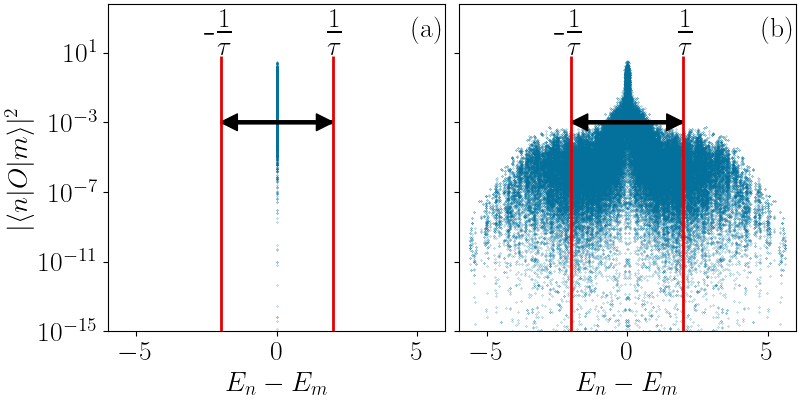
\includegraphics[width=0.8\textwidth]{Figures/cutoff_small.png}
  \caption{Illustration of averaging procedure as defined by equation~\eqref{def:simple time avg}
  for \(\tau = 1/2\). The sum
  of matrix elements is restricted by the \(\theta{}\) function to the region between the two red lines. 
  The operator \(O\) shown here is the \(\hat{O}_1\) as defined in~\eqref{eq:delta 1.0}.
  Matrix elements in panel (a) are calculated for integrable XXZ model~\eqref{eq:XXZ} with \(\Delta = 1\) and in
  panel (b) for the perturbed XXZ model~\eqref{eq:HXXZ perturbed} with \(\Delta = 1\) and perturbation strength
  \(\alpha = 0.1\). Broadening of distribution of matrix elements is the reason why we need finite time averaging
  for investigating nonintegrable systems.}
  \label{fig:cutoff}
\end{figure}
Observing that \({\left(\theta_{mn}^{\tau}\right)}^2 = \theta_{mn}^{\tau}\) and \({\left(\bar{A}^{\tau}\right)}_{mn} =
\theta_{mn}^{\tau} A_{mn}\) we can easily show some crucial properties of time averaging:
\begin{proposition}
  For any \(A,B \in \mathcal{V}_L\)
  \begin{equation*}
    \hs{\bar{A}^{\tau}}{\bar{B}^{\tau}} = \hs{A}{\bar{B}^{\tau}} = \hs{\bar{A}^{\tau}}{B}\;\;\;\;
    \textrm{and}\;\;\;\;
    \overline{\left(\bar{A}^{\tau}\right)}^{\tau} = \bar{A}^{\tau}
  \end{equation*}
  \label{prop:projection}
\end{proposition}
\begin{proof}
  \begin{align*}
    \hs{\bar{A}^{\tau}}{\bar{B}^{\tau}}  & = \frac{1}{\dimension} \sum_{mn} {\left(\bar{A}^{\tau}\right)}_{mn}
    {\left(\bar{B}^{\tau}\right)}_{mn}^{\ast} = \frac{1}{\dimension} \sum_{mn} {\left(\theta_{mn}^{\tau}\right)}^2 A_{mn} B_{mn}^{\ast} \nonumber{}  \\
    & = \frac{1}{\dimension} \sum_{mn} \left(\theta_{mn}^{\tau}\right) A_{mn} B_{mn}^{\ast} =
        \hs{A}{\bar{B}^{\tau}} = \hs{\bar{A}^{\tau}}{B}\\
    \overline{\left(\bar{A}^{\tau}\right)}_{mn}^{\tau} & = {\left(\theta_{mn}^{\tau}\right)}^2 A_{mn} = \theta_{mn}^{\tau} A_{mn} = \left(\bar{A}^{\tau}\right)_{mn}
  \end{align*}  
\end{proof}
These two facts reveal an interesting interpretation of the time averaging, namely, that it can be
thought of as an orthogonal projection in the vector space \(\mathcal{V}_L\). The involutive character of this operation explains,
why we can consider \(\bar{A}^{\tau}\) time independent in the time window \(\left(0,\tau\right)\).

Let us now calculate the commutator of a time-averaged operator with the Hamiltonian
\begin{align}
  \comm{H}{\bar{A}^{\tau}} & = \sum_n \sum_{k,p} E_n \theta_{kp}^{\tau} A_{kp} \comm{ \ketbra{n}{n}}{ \ketbra{k}{p}} \nonumber         \\
                           & = \sum_{k,p} \left(E_k-E_p\right) \theta_{kp}^{\tau} A_{kp} \ketbra{k}{p} \xrightarrow{\tau \to \infty} 0 \label{eq:time averaged commutator}
\end{align}
The last limit follows directly from equation~\eqref{eq:inf time avg}. We can see that the infinite time averaging procedure
creates an integral of motion, i.e. \(\comm{H}{\bar{A}} = 0\). Nonetheless, it is not enough to just time average a
local operator to get a local integral of motion, because in general \(A\in \mathcal{V}_L^M  \nRightarrow \bar{A} 
\in \mathcal{V}_L^M\), that is the truncation of matrix elements modifies the support of an operator.
One possible approach to checking its locality would be to
express this operator in the basis defined in~\eqref{eq:basis}. If for some \(M\) we have \(\bar{A}\in \mathcal{V}_L^M\),
then it is local. Second possibility is that it can be written as a convergent series of operators from \(\mathcal{V}_L^m\) with
increasing \(m\) --- then it is quasilocal. Otherwise, it is a generic nonlocal quantity. But can we do better than this
direct approach?

We begin our journey towards the answer to this question by fixing \(0\leq M \leq L/2\) and constructing a basis \(\{O_s\}\) of \(\mathcal{V}_L^M\). How to actually perform such construction
will be shown in Section~\ref{sec:example}. Next, we find the time averages of all basis operators and build a matrix
\begin{equation}
  K^{\tau}_{st} = \hs{\bar{O_s}^{\tau}}{\bar{O_t}^{\tau}}
  \label{eq:stiffness matrix}
\end{equation}
This matrix is Hermitian by design. However, the models we usually
consider posses time-reversal symmetry, and so we may assume that it is real and symmetric.
The spectral theorem then guarantees the existence of an orthogonal matrix \(U\) that
diagonalizes it. In other words, \(D = UK^{\tau}U^{T}\) is diagonal and we have the following relations
\begin{align}
  &\sum_{s, t} U_{n s} K_{s t}^{\tau} U_{t m}^{T}=\delta_{nm} \lambda_{n} \in
   \RR,\;\;\; \lambda_n \text{ --- eigenvalue of }K^{\tau} \label{eq:property diag} \\
  &UU^{T} = U^{T}U = \mathbb{1} \implies \sum_{s} U_{ns}U_{sm}^{T} =
   \delta_{mn} \label{eq:propery ortho}\\
  & U K^{\tau} = D U \implies \sum_s U_{ns} K_{st}^{\tau} = \sum_s  \delta_{ns} \lambda_s U_{st} = \lambda_n U_{nt}\label{eq:property}
\end{align} 
With the help of the \(U\) matrix (eigenvectors of \(K^{\tau}\)) we can define a new set of rotated operators that
are time-independent in the window \(\left(0,\tau\right)\)
\begin{equation}
  Q_n = \sum_s U_{ns}\bar{O}_{s}^{\tau}\label{eq:new operators}
\end{equation} 

\begin{proposition}
Operators \(Q_n\) are orthogonal, i.e. \(\hs{Q_n}{Q_m} \propto \delta_{nm}\)
\label{prop:orthogonality}
\end{proposition}
\begin{proof}
  Let \(Q_n,Q_m\) be two operators defined as in~\eqref{eq:new operators}.
  Their orthogonality can be shown by direct calculation
  \begin{align*}
    \hs{Q_n}{Q_m} &= \sum_{s,t} U_{ns} {\hs{\bar{O_s}^{\tau}}{\bar{O_t}^{\tau}}} U_{tm}^{T} 
    = \sum_{t} \left(\sum_{s}U_{ns} K_{st}^{\tau}\right)  U_{tm}^{T} \\ 
    &\triangleq \lambda_n \sum_t U_{nt} U_{tm}^{T} \triangleq \lambda_n \delta_{mn}
  \end{align*}
\end{proof}
The last two equalities, marked with \(\triangleq \), follow from properties~\eqref{eq:property} 
and~\eqref{eq:propery ortho} respectively. We can learn something more
about the eigenvalues of \(K^{\tau}\) matrix from a simple corollary to Proposition~\ref{prop:orthogonality}.
\begin{corollary}
  \(K^{\tau}\) is a positive semidefinite matrix.\label{corr:psd}
\end{corollary}
\begin{proof}
Let \(Q_n\) be defined as in~\eqref{eq:new operators}. Then, from the defining properties of the inner product we have that
\(\hs{Q_n}{Q_n} \geq 0\). However, we also have that \(\hs{Q_n}{Q_n} = \lambda_n\). Combining these two equations, we get
that \(\left(\forall n\right) \left(\lambda_n \geq 0\right)\). Therefore \(K^{\tau}\) is a positive semidefinite matrix.
\end{proof}
This corollary provides us with a lower bound on the spectrum of matrix \(K^{\tau}\). 

Let us now examine the support of \(Q_n\). Making use of the basis definition~\eqref{eq:basis},
Proposition~\ref{prop:projection}, and properties~\eqref{eq:property diag},
\eqref{eq:propery ortho},\eqref{eq:property}, we can decompose it into a part supported
on up to \(M\) sites and a nonlocal part
\begin{align}
  Q_n &=  \sum_s \hs{O_s}{Q_n}O_s + Q_s^{\perp} = \sum_{s,t} U_{n t}\hs{O_{s}}{\bar{O}_{t}^{\tau}}
  O_{s}+Q_{n}^{\perp} \nonumber \\
  &= \sum_{s,t} U_{n t}\hs{\bar{O}_{s}^{\tau}}{\bar{O}_{t}^{\tau}} O_{s}+Q_{n}^{\perp}
  = \sum_{s,t} U_{n t}K_{ts} O_{s}+Q_{n}^{\perp} \nonumber \\
  &= \sum_s  \left( \sum_t U_{n t}K_{ts}^{\tau}\right) O_{s}+Q_{n}^{\perp} = \sum_{s} 
  \lambda_{n} U_{n s} O_{s}+Q_{n}^{\perp} = Q_{n}^{M}+Q_{n}^{\perp}
  \label{eq:decomposition}
\end{align}
Now we are ready to derive the central result, stating why this actually algorithm works. 
Combining the fact that \(\hs{Q_n}{Q_n} = \lambda_n \) (see proof of 
Proposition~\ref{prop:orthogonality}) with~\eqref{eq:decomposition} we obtain
\begin{align}
  \lambda_n &= \hs{Q_n}{Q_n} = \hs{Q_n^M + Q_n^{\perp}}{Q_n^M + Q_n^{\perp}} = \hs{Q_n^M}{Q_n^M} +
   \hs{Q_n^{\perp}}{Q_n^{\perp}} + \underbrace{2 \hs{Q_n^M}{Q_n^{\perp}}}_{=0 \text{ (cf.~\eqref{eq:basis})}} \nonumber \\
   &= \hs{\sum_s \lambda_n U_{ns} O_s}{\sum_t \lambda_n U_{nt} O_t} + \norm{Q_n^{\perp}}^2 =
  \lambda_n^2 \sum_{s,t} U_{ns} \hs{O_s}{O_t} U_{tn}^{T} + \norm{Q_n^{\perp}}^2  \nonumber \\
  &=\lambda_n^2 + \norm{Q_n^{\perp}}^2
\end{align}
Rearranging the above equality, we get that \(\lambda_n - \lambda_n^2 = \norm{Q_n^{\perp}}^2 \geq 0\), which together with
Corollary~\ref{corr:psd} gives \(\lambda_n \in \left[0,1\right]\). 

From now on, we shall restrict our considerations to the case \(\tau \to \infty \), 
as it guarantees that \(\bar{O_s}\) and hence \(Q_n\) commutes with the Hamiltonian. 
Consequently, we finally arrive at a classification scheme for the support of \(Q_n\).
\begin{definition}[Classification of IOMs]
  An integral of motion \(Q_n\) is called:
  \begin{itemize}
    \item local: \(\lambda_n = 1 \implies \norm{Q_n^{\perp}} = 0 \implies Q_n \in \mathcal{V}^M_L\)
    \item quasilocal: \(\lambda_n \in \left(0,1\right) \implies \norm{Q_n^{\perp}} > 0 \implies Q_n \in \mathcal{V}_L \)
    \item generic nonlocal: \(\lambda_n = 0 \implies \norm{Q_n} = 0\)
  \end{itemize}
  \label{def:classification}
\end{definition}
The procedure outlined above works for a fixed system size \(L\).
To assess the character of an integral of motion, we need to examine how \(\lambda_n\) 
behaves in the thermodynamic limit. To achieve this, we execute this algorithm for a 
few accessible values of \(L\) and then proceed with finite size scaling.
However, in this thesis we examine both the \(L\to \infty \) case and, depending on
operator, either \(L = 14\) or \(L = 16\)
case, because these are the largest system size for exact diagonalization that we were able to achieve.

It is important not to loose the physical interpretation of these results amidst the formal development.
Operator \(Q_n = \sum_s U_{ns}\bar{O}_{s} = Q_n^M + Q_n^{\perp} \) is always an integral of motion, 
because it is a linear combination of infinite-time averaged operators (cf.~\eqref{eq:time averaged commutator}).
However, the time averaging procedure expands the support of initially local basis operators \(O_s\).
In actual computation we are using the basis of operators supported on up to \(M\) sites at all times, therefore the operator
obtained from the eigenvectors of \(K\) matrix is the \(Q_n^M\) operator. If \(\lambda_n = 1\), then
\(\norm*{Q_n^{\perp}} = 0 \implies Q_n^{\perp} = 0\) and \(Q_n = Q_n^M\). Hence, \(Q_n^M\) operator, which
structure we know, is strictly conserved. On the other hand, if \(\lambda_n \in (0,1) \), then
\(\norm*{Q_n^{\perp}} > 0 \implies Q_n^{\perp} \neq 0\) and \(Q_n \neq Q_n^M\). This means that the operator
that we really get from the algorithm is not a conserved quantity. It is an local approximation, or equivalently
a projection of the true quasilocal integral of motion \(Q_n\) on a basis supported on up to \(M\) sites. Moreover, we can 
construct a convergent series of operators with increasing support and system size, such that their
norm approaches unity. In thermodynamic limit we obtain a strictly conserved
quantity that is \textit{quasilocal}. This discussion motivates a concrete definition
of quasilocality~\footnote{Some authors refer to this condition as \textit{pseudolocality},
while reserving the name \textit{quasilocality} for a stronger condition. For details
see~\textcite{Ilievski2016a}.}~\autocite{Mierzejewski2020b}
\begin{definition}[Quasilocality]
A conserved operator \(Q\in \mathcal{V}_L\) is called quasilocal, if for some \(M\in \NN\)
there exist a local operator \(A \in \mathcal{V}_L^M \), such that
\begin{equation*}
  \lim_{L\to \infty} \frac{\hs{Q}{A}}{\hs{Q}{Q}} > 0
\end{equation*}
i.e.\ \(Q\) has finite overlap with \(A\) in thermodynamic limit.
  \label{def:formal quasilocal}
\end{definition}
If \(\norm*{Q_n^{\perp}} > 0\), and \(\lim_{L\to \infty} \lambda_n \neq 0\),
then the \(Q_n^M\) operator obtained from the algorithm is precisely the local operator from
definition~\ref{def:formal quasilocal}.
We will end the discussion about the algorithm with 
a short summary on support of \(Q_n\):
\begin{align}
  & Q_n = Q_n^M + Q_n^{\perp}\nonumber\\
  & \norm*{Q_n}^2 = \lambda_n \nonumber\\
  & \norm*{Q_n^M}^2 = \lambda_n^2 \nonumber\\
  & \norm*{Q_n^{\perp}}^2 = \lambda_n - \lambda_n^2
  \label{eq:summary of support}
\end{align}

\paragraph{Proof of correctness}
Suppose we have an operator \(\mathcal{V}_L^M \ni A = \sum_s u_s O_s \), where \(u_s \in \RR \) for all \(s\).
We can identify this operator from \(\mathcal{V}_L^M\) with a vector \( \bm{u} \in \RR^{\dim{\mathcal{V}_L^M}}\). Using this picture,
the stiffness of \(A\) can be calculated as follows
\begin{equation}
  \hs{\bar{A}}{\bar{A}} = \sum_{s,t} u_s \hs{\bar{O}_s}{\bar{O}_t} u_t = \sum_{s,t} u_s K_{st} u_t = 
   \bm{u}^{T} K \bm{u}  
\end{equation} 
Thus, the problem in quantum mechanics is reduced to the problem in linear algebra.
Because all eigenvalues of \(K\) matrix are real, we can sort the corresponding operators
 (defined by columns of \(U\) matrix, i.e.\;eigenvectors of \(K\)) by their magnitude.
We then say that the larger the eigenvalue, the `better' the integral of motion is, i.e.\
it has larger projection on a local basis.
But can we be sure that the maximal eigenvalue obtained from the algorithm corresponds
to the `best' possible integral of motion? To put it another way, if the procedure detects
neither local nor quasilocal integrals of motion, does that necessarily mean they do not exist
for a given system? The answer to this question lies within the subsequent
\begin{proposition}
Let \(\lambda \) be the maximal eigenvalue of \(K\). Then the following equality holds
\begin{equation*}
  \lambda = \max_{  \substack{\bm{v}\in \RR^{\dim{\mathcal{V}_L^M}}\\\norm{v} = 1}  }{\bm{v}^{T} K \bm{v}}
\end{equation*}
\end{proposition}
\begin{proof}
  Assume the converse, i.e.\ there exists such \(\bm{u} \in \RR^{\dim{\mathcal{V}_L^M}}\) that \(\bm{u}^T K \bm{u} > \lambda\)
  and \(\norm{\bm{u}} = 1\).
  Let \(\set{\bm{v}_n}\) be a orthonormal basis consisting of eigenvectors of \(K\). We can express \(\bm{u}\) in this basis as
  \(\sum_n u_n \bm{v}_n\) for \(u_n \in \RR\). Then we have:
  \begin{align*}    
    \bm{u}^T K \bm{u} &= \left( \sum_n u_n \bm{v}_n^{T} \right) K  \left( \sum_m u_m \bm{v}_m \right) 
    = \sum_{n,m} u_n u_m \lambda_m \underbrace{\bm{v}_n^{T} \bm{v}_m}_{\delta_{mn}} \\
    &= \sum_n u_n^2 \lambda_n \leq \sum_n u_n^2 \lambda = \lambda \sum_n u_n^2 = \lambda   
  \end{align*}
  Obtained contradiction concludes the proof.
\end{proof}

%%%%%%%%%%%%%%%%%%%%%%%%%%%%%%%%%%%%%%%%%%%%%%%%%%%%%%%%%%%%%%%%%%%%%%%%%%%%%%%%%%%%%%%%%%%%%%%%%%%%%%%%%%%%%%%%%%%%%%%%%%%%%%%

\section{Spectral functions and Mazur bound\label{sec:spectral function}}

\paragraph{Spectral functions}After we have learned about local and quasilocal IOMs and how to find them, it is perhaps the 
time to ask why are they actually important. To answer this question in a convincing manner we 
follow the discussion in~\textcite{Vidmar2021} and introduce the concept of spectral
function. 

Suppose that we have a real observable \(A \in \mathcal{V}_L^M\) and we are interested in studying its time
evolution. An obvious choice would be to calculate its autocorrelation function
\((A(t)|A)\), where the time dependence of \(A(t)\) is understood
via the Heisenberg picture i.e.\ \(A(t) = \exp\left(i H t\right) A
\exp\left(-i H t\right)\). However, this quantity is rather unpleasant to work with.
Instead, we shall investigate the Fourier transform of the autocorrelation function, formally
defined as
\begin{definition}[Spectral function]  
  \begin{equation*}
  S(\omega) =  \lim _{\varepsilon \to 0^+} \frac{1}{2 \pi} \int_{-\infty}^{\infty} \mathrm{d} t 
  \; \mathrm{e}^{i \omega t-|t| \varepsilon}\hs{A(t)}{A}
  \end{equation*}
  \label{def:spectral function}
\end{definition}
The limit in the definition is present to ensure proper convergence of the integral
and \(\omega{}\) corresponds to \(\frac{1}{\tau}\) from earlier discussion.
To connect this quantity with numerical calculations and to smoothen out any fluctuations, we
can once again integrate it, but this time over a finite frequency window
\begin{equation}
  I(\omega) = \int_{-\omega}^{\omega} \mathrm{d}\omega^{\prime} \; S(\omega^{\prime}) = 
  \frac{1}{\dimension} \sum_{m,n} \theta\left(\omega - |E_m-E_n|\right) A_{mn}^2
  \label{eq:integrated spectral function}
\end{equation}
For the derivation of equation~\eqref{eq:integrated spectral function} see Appendix~\ref{app:spectral}.
It turns out that this quantity is equal to the square of Hilbert-Schmidt norm of time
averaged operator \(\bar{A}^{\frac{1}{\omega}}\), which fits nicely within the previously
discussed framework. Because all observables of interest are traceless and
normalized to unity, we have these two important limits
\begin{align}
  \lim_{\omega \to \infty } I(\omega) &= \frac{1}{\dimension}\sum_{m,n} A_{mn}^2 = \norm*{A}^2 = 1\\
  \lim_{\omega \to 0^+ } I(\omega) &= \frac{1}{\dimension} \sum_{ \substack{m,n\\E_m=E_n} } A_{mn}^2 = \norm*{\bar{A}}^2
\end{align}

For frequencies small (long times) in comparison with the system's characteristic energy
scale, spectral function of an observable \(A \in \mathcal{V}_L^M\) can be approximated as follows
\begin{equation}
  S(\omega \ll  J) \simeq  D_{A} \delta(\omega)
  \label{eq:spectral approximation}
\end{equation}
where \(D_A = \lim_{\omega\to 0^+} I(\omega) = \hs{\bar{A}}{\bar{A}}\) is the stiffness of \(A\).
Let us now imagine that we have a complete set of orthogonal (Q)LIOMs 
\(\hs{Q_{n}}{Q_{m}} \propto \delta_{nm}\). It was shown 
by~\textcite{Mazur1969,Suzuki1971} that the stiffness \(D_{A}\) of arbitrary observable \(A\) has its origin
in the projections on these \(Q_{n}\)
\begin{equation}
  D_A = \sum_{n} D_{n} = \sum_{n} \frac{\hs{A}{Q_{n}}^2}
  {\hs{Q_{n}}{Q_{n}}}
  \label{eq:mazur equality}
\end{equation}
Therefore, by calculating the overlap between our observable and all (Q)LIOMs, we can infer about the long time
behavior of its spectral function and thus its autocorrelation function. It is here that the
importance of (Q)LIOMs becomes evident, as the overlap with generic nonlocal conserved quantities
vanishes in the thermodynamic limit~\autocite{Zotos1997}.
Because autocorrelation function of
LIOMs is constant, its Fourier transform is a Dirac delta, which explains the form of 
equation~\eqref{eq:spectral approximation}. 

\paragraph{Mazur bound} If we know only a subset of the full set of (Q)LIOMs, 
equality~\eqref{eq:mazur equality} turns into 
a very useful lower bound for stiffness, called the \textit{Mazur bound}. We will now proceed with a derivation
of this bound for the case of one (Q)LIOM, in the spirit of a more modern discussion from~\textcite{Ilievski2016a}.
\begin{proposition}[Mazur bound for a single (Q)LIOM]
  Let \(A\in \mathcal{V}_L^M\) be an arbitrary observable and \(Q\) be a (quasi)local conserved quantity. Then the following inequality
  holds
  \begin{equation*}
    D_{A} = \hs{\bar{A}}{\bar{A}} \geq \frac{\hs{A}{Q}^2}{\hs{Q}{Q}} > 0
  \end{equation*}
  \label{prop:single mazur}
\end{proposition}

\begin{proof}
  We define a new observable \(\mathcal{A} = \bar{A} - \alpha Q\) for \(\alpha \in \RR\).
  Clearly, square of the norm of this quantity is positive i.e. \(\norm*{\mathcal{A}}^2 = 
  \tr(\mathcal{A}\mathcal{A})/\dimension \geq 0\). On the other hand, we can carry out an
  explicit computation of the norm
  \begin{align*}
  \norm*{\mathcal{A}}^2 &= \hs{\bar{A}-\alpha Q}{\bar{A}-\alpha Q} = \hs{\bar{A}}{\bar{A}} - 
  \hs{\bar{A}}{Q} - \alpha \hs{Q}{\bar{A}} + \alpha^2 \hs{Q}{Q} \\
  &= \hs{\bar{A}}{\bar{A}} - 2\alpha \hs{A}{Q} + \alpha^2 \hs{Q}{Q} \geq 0
  \end{align*}
  Between the first and the second line we have used the fact that \(\hs{\bar{A}}{\bar{B}} = 
  \hs{\bar{A}}{B} = \hs{A}{\bar{B}}\)(cf. Proposition~\ref{prop:projection}) and \(\bar{Q} = Q\) 
  for a conserved quantity. Let us now substitute \(\alpha = \frac{\hs{A}{Q}}{\hs{Q}{Q}}\) to the
  above inequality.
  \begin{align*}
    D_A = \hs{\bar{A}}{\bar{A}} &\geq 2 \frac{\hs{A}{Q}}{\hs{Q}{Q}} \hs{A}{Q} - \frac{\hs{A}{Q}^2}{\hs{Q}{Q}^2}\hs{Q}{Q}
    = \frac{\hs{A}{Q}^2}{\hs{Q}{Q}} > 0
  \end{align*}
  The last equality follows from Definition~\refeq{def:formal quasilocal} and (quasi)locality of Q.
  \label{proof:single mazur}  
\end{proof}
It is perhaps worth noting that the derivation Mazur bound for a single (Q)LIOM is almost equivalent to the proof of
the Cauchy-Schwartz inequality, found in any linear algebra textbook. By following exactly the same procedure, 
we can easily generalize this result to a set of orthogonal conserved quantities \(\{Q_{n}\}\)
\begin{equation}
  D_A = \hs{\bar{A}}{\bar{A}} \geq \sum_{n} \frac{\hs{A}{Q_n}^2}{\hs{Q_n}{Q_n}}
\end{equation}

We have already seen that Mazur inequality turns into an equality, if the set \(\{Q_n\}\) is complete. However,
up until a few years ago, it was not clear how to systematically identify such a complete set in interacting models.
This have changed with the work of~\textcite{Mierzejewski2015a}, where the algorithm described in details
in Section~\ref{sec:algorithm} was first proposed. We shall now show that the following proposition holds~\autocite{Mierzejewski2015Approx}
\begin{proposition}[Saturation of Mazur bound]
  The set \(\{Q_n\}\) of (Q)LIOMs obtained from the algorithm in Section~\ref{sec:algorithm} is complete,
  that is it saturates the Mazur bound. 
\label{prop:saturation}
\end{proposition}
\begin{proof}
  Consider once again an arbitrary observable \(\mathcal{V}_L^M \ni A = \sum_n a_n O_n,\; 
  (\forall n) (a_n \in \RR)\). We are interested in computing its stiffness \(D_A = \hs{\bar{A}}{\bar{A}}\), 
  where \(\bar{A} = \sum_n a_n \bar{O}_n\). Inverting the relation~\eqref{eq:new operators}, we can write 
  \(\bar{O}_n = \sum_s U_{ns}^T Q_s = \sum_s U_{sn} Q_s\) and thus the following
  \begin{equation*}
    \bar{A} = \sum_n a_n \bar{O}_n = \sum_n a_n \sum_s U_{sn} Q_s =
    \sum_s \underbrace{\left(\sum_n a_n U_{sn}\right)}_{v_s} Q_s = \sum_s v_s Q_s
  \end{equation*}
  Now, let us express the overlap \(\hs{\bar{A}}{Q_k}\) in two ways
  \begin{enumerate}
    \item \(\hs{\bar{A}}{Q_k} = \sum_s v_s \underbrace{\hs{Q_s}{Q_k}}_{=\lambda_s \delta_{sk}} = v_k \lambda_k\)
    \item \(\hs{\bar{A}}{Q_k} = \hs{A}{\bar{Q_k}} = \hs{A}{Q_k}\)
  \end{enumerate}
  We are finally ready to make a direct calculation of stiffness of \(A\)
  \begin{align*}
    D_A = \hs{\bar{A}}{\bar{A}} &= \sum_{sk} v_s v_k \hs{Q_s}{Q_k} = \sum_{sk} v_s v_k \delta_{sk} \lambda_{k} = 
    \sum_{\substack{s\\\lambda_s > 0}} v_s^2 \lambda_s \\
    &= \sum_{\substack{s\\\lambda_s > 0}} v_s^2 \lambda_s^2 \frac{1}{\lambda_s} = 
    \sum_{\substack{s\\\lambda_s > 0}} \frac{\hs{A}{Q_s}^2}{\hs{Q_s}{Q_s}}
  \end{align*}
  Therefore, the Mazur bound is saturated by our construction and the proof is completed.
\end{proof}
We finish this section with an example of an application of Mazur bound. 
\begin{example}
  Consider the topic of ballistic linear response~\autocite{Ilievski2016a}. Let \(J\) be an extensive current,
  for example the spin current. From Kubo linear response theory
  we have the following well-known expression for the real (non-dissipative) part of dynamical
  spin conductivity~\autocite{Zotos1996}
  \begin{equation}
    \sigma'(\omega) = 2 \pi D_J \delta(\omega) + \sigma_J^{reg}(\omega)
  \label{eq:conductivity}
  \end{equation}
If there exists a (quasi)local conserved quantity \(Q\) such that \(\hs{J}{Q}>0\), the Mazur bound
implies that \(D_J > 0\). Such a nonzero value of spin current stiffness is an indicator of \textit{ballistic}
DC transport (i.e.\ without scattering, cf. Figure~\ref{fig:spin transport}) --- \(\sigma'(0)\) diverges. 
\end{example}
\begin{figure}[htbp]
  \centering
  \begin{tikzpicture}[scale=1.4]
    \colorlet{col1}{blue!30}
  
   \begin{scope}[smooth,draw=gray!20,y=0.3989422804cm]
        \filldraw[fill=col1] plot[id=f1, domain=-1.5:1.5,samples=100] function {6*exp(-6*x*x)};
        \draw[black] plot[id=f2,domain=-1.5:1.5,samples=100]
            function {6*exp(-6*x*x)};
    \end{scope}
    \draw[->] (-1.5,0) -- (1.5,0) node [right] {$x$};
    \draw[->] (-1.5,0) -- (-1.5,2.5) node [midway,rotate=90,yshift=6pt] {spin density};
    \draw[<->] (-0.37,1) -- (0.37,1) node [midway, yshift=6pt] {$\gamma$};
  
    \begin{scope}[smooth,draw=gray!20,y=0.3989422804cm]  
      \draw[black] plot[id=f3,domain=2.35:5.35,samples=100] function {0.7};    
      \draw[black] plot[id=f4,domain=2.35:5.35,samples=100] function {x};    
      \draw[black] plot[id=f5,domain=2.35:5.35,samples=100] function {sqrt(x)};    
    \end{scope}  
    
    \draw[->] (2.35,0) -- (5.35,0) node [right] {$t$};
    \draw[->] (2.35,0) -- (2.35,2.5) node [right] {$\gamma$};
    \node[draw=none] at (3.35,1.6) {$\gamma \propto t$};
    \node[draw=none] at (3.45,0.95) {$\gamma \propto \sqrt{t}$};
    \node[draw=none] at (3.6,0.4) {$\gamma = const$};
    \node[draw=none] (localized) at (6,0.3) {localized};
    \node[draw=none,above of=localized,node distance=27pt] (diffusive) {diffusive};
    \node[draw=none,above of=diffusive,node distance=45pt] (ballistic) {ballistic};
  \end{tikzpicture}  
  \caption{Illustration of different types of transport. On the left panel, we have some initial spin
  density characterized by width \(\gamma\). On the right panel, we have the dependence of \(\gamma\)
  on time in three different cases.}
  \label{fig:spin transport}
\end{figure}

%%%%%%%%%%%%%%%%%%%%%%%%%%%%%%%%%%%%%%%%%%%%%%%%%%%%%%%%%%%%%%%%%%%%%%%%%%%%%%%%%%%%%%%%%%%%%%%%%%%%%%%%%%%%%%%%%%%%%%%%%%%%%%%%

\section{(Q)LIOMs supported on up to \(3\) sites in the XXZ model\label{sec:example}}

After explaining how and why to look for LIOMs and QLIOMs, let us now turn to a more concrete
example of spin-\(1/2\) XXZ model on one-dimensional lattice of \(L\) sites with periodic
boundary conditions, introduced already in Section~\ref{sec:XXZ}. The subsequent
considerations are based on the work of~\textcite{Mierzejewski2015a}.

Having chosen a concrete model, we can now give an explicit definition of a basis
of a space of \(m\)-local observables \(\mathcal{V}_L^m\). It is composed of operators
of the form
\begin{equation}
  O_{\underline{s},j}=\sigma_{j}^{s_{1}} \sigma_{j+1}^{s_{2}} \cdots 
  \sigma_{j+m-1}^{s_{m}}
  \label{eq:basis operator}
\end{equation}
In the expression above we have \(\sigma_j^z \equiv 2 S^z_j\),
\(\sigma_j^{\pm} \equiv \sqrt{2} S_j^{\pm}\), \(\sigma^{0}_j \equiv \Id_{2\cross 2}\) and
 \(\underline{s} = \left(s_1, s_2,\ldots, s_m\right)\) where \(s_j \in \{+,-,z,0\}\) for
 \(j \in \{2,3,\ldots,m-1\}\). For the first and the last operator in a sequence we have 
 \(s_{1,m} \in \{+,-,z\}\), because the identity there would correspond to an \((m-1)\)-local
 operator. The index \(j\) indicates the first site of support.
As a matter of mathematical precision, the notation for \(O_{\underline{s},j}\) used here 
(and frequently in the physics literature) is a bit of simplification. It is important to remember
that because of embedding~\eqref{eq:embedding}, there are tensor products between \(\sigma_j\), i.e.\ we have the following
\begin{equation}
  O_{\underline{s},j}= \underbrace{\Id_{2\cross 2} \otimes \cdots
       \otimes \Id_{2\cross 2}}_{j-1} \otimes \; \sigma_{j}^{s_{1}} \otimes \sigma_{j+1}^{s_{2}} \otimes
        \cdots \otimes \sigma_{j+m-1}^{s_{m}} \otimes 
        \underbrace{\Id_{2\cross 2} \otimes \cdots \otimes \Id_{2\cross 2}}_{L-j-m+1}
        \label{eq:basis with tensors}
\end{equation}
The single site identity operators ensure that the dimension of matrix of the operator is right.
A simple combinatorial observation shows us that there are \(N_m = 3\cdot 4^{m-2}\cdot 2\)
(excluding shifts, i.e.\ different values of \(j\) for the same \(\underline{s}\)) operators
constituting a \(m\)-local basis (for \(m = 1\) we have \(N_1 = 3\)). Moreover, they are orthonormal
\textit{by design}, i.e.\ \(\hs{O_{\underline{s},j}}{O_{\underline{s}^{\prime}},j^{\prime}} =
\delta_{\underline{s},\underline{s}^{\prime}}\delta_{j,j^{\prime}}\) (see Appendix~\ref{app:orthonormality} for proof).
Fixing \(M>0\) (usually \(M<L\)), we can construct the basis of traceless operators spanning
the space \(\mathcal{V}_L^M = \bigoplus_{m=1}^{M} \mathcal{V}_L^m\). From the properties of 
direct sum of linear spaces, we now see that its cardinality is \(D_M = \sum_{m=1}^{M} N_m = 
 3 \cdot 4^{M-1}\). To include all possible shifts, this value needs to multiplied by
 the number of sites \(L\). Such construction can be implemented in practice by considering
 all possible \(M\)-digit numbers written in base \(4\) (as there are \(4\) `building blocks':
  \(\sigma^{+},\sigma^{-},\sigma^{z},\Id_{2\cross 2}\)). 

Having put together this basis, we can now proceed with the rest of the (Q)LIOM finding algorithm.
However, before that it is beneficial to discuss the influence of the symmetries of the system in question,
the XXZ model. They allow us to decompose the matrix \(K\) 
(cf.~\eqref{eq:stiffness matrix}) and usually reduce the computational effort. First and perhaps
the most important one is implied by the fact already discussed in Section~\ref{sec:prelim} ---
conservation of magnetization. We could restrict our considerations to a subspaces
of \(\mathcal{V}_L^M\) comprised of operators such that \(\comm{S_{tot}^z}{O_{\underline{s}}} = 0\).
Yet, we will not be able to use that symmetry here, as in this work we are interested 
in the \textit{noncommuting} operators, i.e\ precisely those that break this symmetry.
Furthermore, the XXZ model is time-reversal invariant, so the \(K\) matrix is real and symmetric.
Therefore, we can divide our operators into two orthogonal subspaces, either real or imaginary.
Those subspaces are then spanned by operators of the form 
\(O_{\underline{s}}+O^{\dagger}_{\underline{s}}\) or 
\(i(O_{\underline{s}}-O^{\dagger}_{\underline{s}})\) respectively. There is also one more
useful symmetry, namely the \(\ZZ_2\) spin-flip symmetry, however it remains out scope of
this thesis. 


%%%%%%%%%%%%%%%%%%%%%%%%%%%%%%%%%%%%%%%%%%%%%%%%%%%%%%%%%%%%%%%%%%%%%%%%%%%%%%%%%%%%%%%%%%%%%%%%%%%%%%%%%%%%%%%%%%%%%%%%%%%%%%%%
\subsection{Commuting LIOM: Spin energy current\label{sec:energy current}}
In order to test our (Q)LIOM finding algorithm and the correctness of its implementation, we first
investigate the known case of energy current in Spin\(-1/2\) XXZ model~\autocite*{Mierzejewski2015Approx}
and see whether it is detected or not. For the sake of completeness, derivation of
spin energy current for the general XYZ model is be presented, following the definitions in \textcite{Zotos1997}.
We start with the general XYZ Hamiltonian with periodic boundary conditions~\eqref{eq:XYZ}.
It is easy to see that this Hamiltonian can be represented as a sum of operators supported on two consecutive sites
\begin{equation}
  H_{XYZ} = \sum_{k=1}^L h_{k,k+1}
\end{equation}
where \(h_{k,k+1} = J_{x} \Sx_{k}\Sx_{k+1} + J_{y} \Sy_{k}\Sy_{k+1} + J_{z} \Sz_{k}\Sz_{k+1} \) and periodic boundary conditions
require that \(h_{L,L+1} = h_{L,1}\). The energy operator is a conserved quantity, thus the time evolution of its local density
is given by the discrete continuity equation
\begin{equation}
  \dv{h_{k,k+1}(t)}{t} + \div{j_{k}^{E}(t)} = 0
  \label{eq:discrete continuity}
\end{equation}
where \(\div{j_{k}^E(t)} \equiv j_{k+1}^E(t) - j_{k}^E(t)\) is the discrete divergence of spin energy current density and \(h_{i,i+1}(t) = \mathrm{e}^{i H_{XYZ}t} h_{i,i+1} \mathrm{e}^{-i H_{XYZ} t}\).
On the other hand, the time evolution of an arbitrary operator is determined
by the Heisenberg equation
\begin{equation}
  \dv{h_{k,k+1}(t)}{t} = i \comm{H_{XYZ}}{h_{k,k+1}(t)}
  \label{eq:heisenberg equation}
\end{equation}
Combining equations~\eqref{eq:discrete continuity} and~\eqref{eq:heisenberg equation} we obtain the defining equations for
the spin energy current density
\begin{equation}
  j_{k+1}^E - j_{k}^E = - i \comm{H_{XYZ}}{h_{k,k+1}} = i \comm{h_{k,k+1}}{H_{XYZ}} = i \sum_{r=1}^L \comm{h_{k,k+1}}{h_{r,r+1}}
  \label{eq:energy current defining equation}
\end{equation}
Similar equations can be written for any operator being a sum of local operators such as
the total spin operator or particle number operator in fermionic models. Detailed solution to equation~\eqref{eq:energy current defining equation}
is shown in Appendix~\ref{app:spin energy current derivation}. For the XXZ model, we get the following expression
\begin{align*}
  j_k^E & = i \Big( \underbrace{2J \Sm_{k-1}\Sz_k \Sp_{k+1} + J \Delta \Sz_{k-1}\Sp_k \Sm_{k+1} + J\Delta \Sp_{k-1}\Sm_k\Sz_{k+1}}_{O_k}                                  \\
        & - \underbrace{\left(2J \Sp_{k-1}\Sz_k \Sm_{k+1} + J\Delta \Sz_{k-1}\Sm_k \Sp_{k+1} + J\Delta \Sm_{k-1}\Sp_{k} \Sz_{k+1} \right)}_{O_k^{\dagger}}\Big) \nonumber \\
        & = i\left(O_k - O_k^{\dagger}\right)
\end{align*}
Thus we see that it is an imaginary operator. Moreover, it is also a commuting operator
because it consists of a sum of equal number of \(\Sp{}\) and \(\Sm{}\). 
Obtaining the energy current operator is now simply the matter of summing over all lattice sites
\begin{equation}
  J^E = \sum_{k=1}^L j_k^E
  \label{eq:energy current}
\end{equation}
As the energy current commutes with the Hamiltonian~\autocite{Zotos1997}, it does not undergo time evolution
and its autocorrelation function \(\hs{J^E(t)}{J^E(0)}\) is constant. Therefore, the corresponding
spectral function is proportional to Dirac delta.
\begin{figure}[htbp]
  \centering
  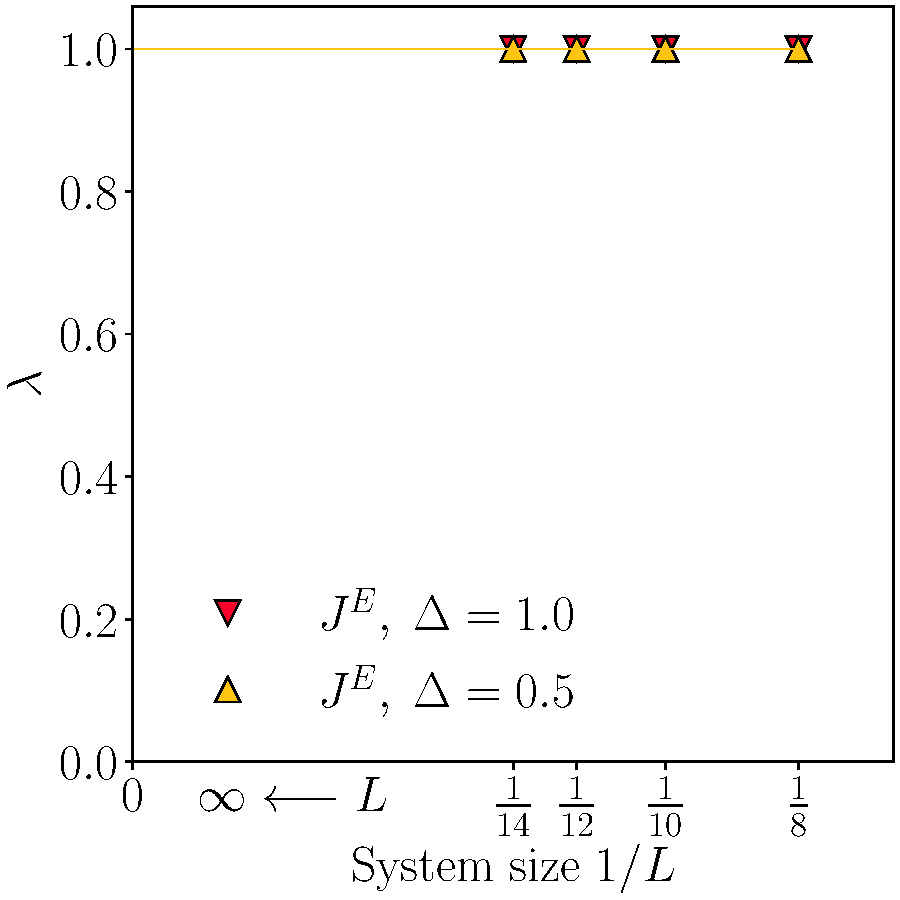
\includegraphics[width=0.5\textwidth]{Figures/current_int.pdf}
  \caption{Eigenvalues of generalized stiffness matrix corresponding to the energy current
  operator as a function of inverse system size. Solid line is the extrapolation to thermodynamic
  limit. Calculations performed for \(\Delta=1.0\) and \(\Delta=0.5\).}\label{fig: current integrable}
\end{figure}
After restricting our algorithm to the case of imaginary
operators, we obtain the following
\begin{equation}
    J^E = \sum_{k=1}^L i\left[\beta_1 \left(\Sm_{k-1}\Sz_{k}\Sp_{k+1}\right) + \beta_2 \left(\Sz_{k-1}\Sp_{k}\Sm_{k+1}+\Sp_{k-1}\Sm_{k}\Sz_{k+1}\right)\right] + \text{H.c.}
\end{equation}
where the coefficients \(\beta_1,\beta_2\) are such that the operator is properly
normalized. This is precisely the energy current operator as derived above.
After taking the thermodynamic limit of the eigenvalue of \(K\) matrix 
corresponding to the energy current, we see that it equals one (Figure~\ref{fig: current integrable}).
Thus, according to Definition~\ref{def:classification}, it is a local integral of motion. 

%%%%%%%%%%%%%%%%%%%%%%%%%%%%%%%%%%%%%%%%%%%%%%%%%%%%%%%%%%%%%%%%%%%%%%%%%%%%%%%%%%%%%%%%%%%%%%%%%%%
\subsection{Noncommuting (Q)LIOMs\label{subsec:noncomm qlioms}}
Having checked the correctness of the algorithm and its implementation, we can now proceed with the
main topic of this thesis, that is, investigating the \textit{noncommuting} integrals of motion. 
We conducted preliminary studies for small values of system size \(L\), without assuming
translational invariance. Available resources allowed us to make an unrestricted search for
 \(L \in \set{8,9,10,11,12}\). Nevertheless, the noncommuting operators that maximized stiffness for given 
 \(L\) and \(\Delta \) turned out to be either translationally invariant or translationally invariant with
 a sign flip (see \(\hat{O}_2\)~\eqref{eq:delta 0.5}). Therefore, we restricted our further 
considerations to such operators only. This allowed us to quite easily obtain numerical
results for \(L\) up to \(14\). After quite lengthy calculations, we were also able
to obtain some results for \(L=16\).
We will focus on two concrete cases of operators, corresponding
to largest eigenvalues of the generalized stiffness matrix for values of anisotropy
parameter \(\Delta=1.0\) and \(\Delta=0.5\) respectively. For this values of
\( \Delta \) parameter, the many-body energy spectrum exhibits massive degeneracies, because
eigenstates with different \(\Sz_{tot}\) correspond to the same energies~\autocite{Fagotti2014,Mierzejewski2021}.

For the case of \(\Delta=1.0\), the XXZ model reduces to the isotropic Heisenberg model~\eqref{eq:XXX}
possessing \(SU(2)\) symmetry.
As a consequence of this symmetry, the conservation of total magnetization 
(\(\Sz_{tot}\) operator~\eqref{eq:magnetization}) implies the conservation of analogously defined \(\Sx_{tot}\)
and \(\Sy_{tot}\) and therefore the following quantity
\begin{equation}
    \hat{O}_{1} =  \frac{1}{\sqrt{L}}\sum_{j=1}^{L} \Sp_{j} + \text{H.c.}
    \label{eq:delta 1.0}
\end{equation}
where the prefactor is introduced for the sake of normalization. Note that
this operator is actually the \(\Sx_{tot}\), however this form shows that \(\hat{O}_1\) 
is an example of a real operator. If we were to consider an analogously defined imaginary operator,
we would obtain the \(\Sy_{tot}\), but due to \(SU(2)\) symmetry results would be the same.


The case of \(\Delta=0.5\) is much more difficult. It was shown by~\textcite{zadnik2016} that for 
special values of anisotropy parameter \(\Delta \in S = \set[\Big]{\cos\left(\frac{2l}{2k-1}
\pi\right)}_{k,l\in \NN,\, l<k}\) one can use semicyclic irreducible representations
of quantum group \(U_q(\mathfrak{sl}_2)\) to generate a set of quasilocal integrals of 
motion that do not preserve magnetization. Even though the set \(S\) is a dense subset
of the interval \([-1,1]\) i.e.\ the gapless regime of XXZ spin-\(1/2\) chain, it is not
symmetric with respect to \(\Delta=0\). For example, considered here value of anisotropy parameter
\(\Delta=0.5\) does not belong to this set, whereas \(\Delta=-0.5\) do. However, it can be shown
that for even system sizes, in thermodynamic limit, there exists a unitary operator 
\(U = \left(\Id_{2\cross 2}\otimes \tau^z\right)^{\otimes L/2}\), which action is equivalent to flipping the sign 
of parameter \(\Delta\), that is \(UH_{XXZ}(\Delta)U = -H_{XXZ}(-\Delta)\). It follows then,
that if \(Q\) is a conserved quantity for \(\Delta\), then \(\tilde{Q} = UQU\) is a conserved
quantity for \(-\Delta\). This is the reason we present numerical results only for even 
values of \(L\). For \(\Delta=0.5\) the action
of this operator produces a simple factor of \((-1)^i\) and the operator of interest reads
\begin{equation}
  \hat{O}_{2} =\frac{1}{\sqrt{L}} \sum_{j=1}^{L} {(-1)}^j \left( \Sp_{j}\Sp_{j+1}\Sp_{j+2}\right) + \text{H.c.}
  \label{eq:delta 0.5}
\end{equation}  
This is once again a real operator. Detailed discussed of this topic is far beyond the scope of this thesis
and can be found in~\autocite{Ilievski2016a,zadnik2016,Prosen2014c}.

\begin{figure}[htbp]
  \centering
  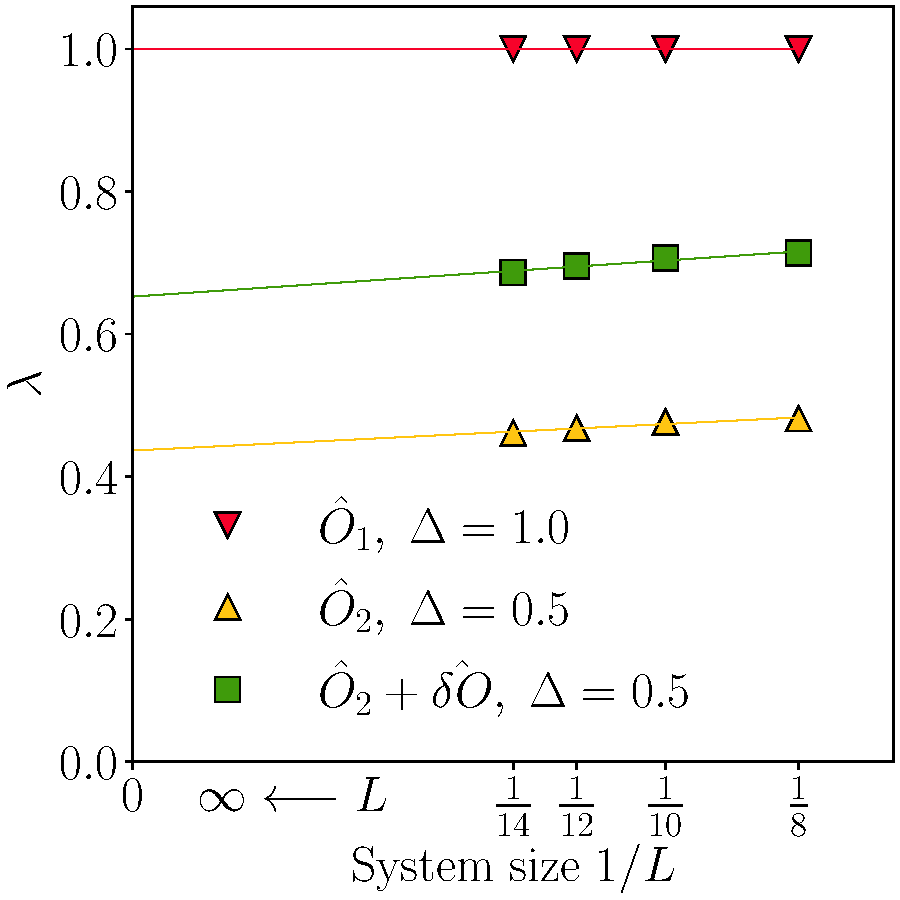
\includegraphics[width=0.5\textwidth]{Figures/nocomm_int.pdf}
  \caption{Eigenvalues of generalized stiffness matrix corresponding to the two noncommuting
    integrals of motion, as a function of inverse system size. Solid lines represent the extrapolation
    to the thermodynamic limit. Note that the operator \(\hat{O}_2\) exhibits quasilocality
    and its stiffness in the thermodynamic limit is \(\lambda_{L\to\infty} \approx
    0.43\). Stiffness of \(\hat{O}_2 + \hat{\delta O}\) in thermodynamic limit is
    \(\lambda_{L\to\infty} \approx 0.65\)}
  \label{fig: noncommuting integrable}
\end{figure}

Both \(\hat{O}_1\) and \(\hat{O}_2\) are noncommuting operators, what can be seen easily from the
fact that they consist of products of either just \(\Sp\) operators or \(\Sm\) operators. Conducting
an analysis with the help of the algorithm, we indeed find these two operators among eigenvectors
of the generalized stiffness matrix. Corresponding eigenvalues and their thermodynamic limit
are shown in Figure~\ref{fig: noncommuting integrable}. Comparing it with 
Definition~\ref{def:classification} we see that \(\hat{O}_1\) is a strictly 
conserved, local integral of motion, whereas \(\hat{O}_2\) is a projection 
of a quasilocal integral of motion on a basis supported on up to \(3\) sites.
To further illustrate the concept of quasilocality, we can consider a projection
of this QLIOM on a basis supported on up to \(4\) sites, which results in an operator of the form 
\(\hat{O}_2 + \hat{\delta O}\), where \(\hat{\delta O}\) is the complicated \(4\)-local part.
Looking at Figure~\ref{fig: noncommuting integrable} we see
that stiffness of this new projection is larger than that of the old one. However, contribution 
of \(\hat{\delta O}\) to the overall stiffness is smaller than that of \(\hat{O}_2\).
